\documentclass[12pt]{article}
\usepackage{amsmath}
\usepackage{graphicx,psfrag,epsf}
\usepackage{enumerate}
\usepackage{natbib}
\usepackage{url} % not crucial - just used below for the URL 
\usepackage[labelfont=bf,font=bf]{caption}
%\pdfminorversion=4
% NOTE: To produce blinded version, replace "0" with "1" below.
\newcommand{\blind}{0}

% DON'T change margins - should be 1 inch all around.
\addtolength{\oddsidemargin}{-.5in}%
\addtolength{\evensidemargin}{-.5in}%
\addtolength{\textwidth}{1in}%
\addtolength{\textheight}{.8in}%
\addtolength{\topmargin}{-1in}%


\begin{document}
{\fontsize{2.5}{4}\selectfont}
%\bibliographystyle{natbib}

% \def\spacingset#1{\renewcommand{\baselinestretch}%
% {#1}\small\normalsize} \spacingset{1}


%%%%%%%%%%%%%%%%%%%%%%%%%%%%%%%%%%%%%%%%%%%%%%%%%%%%%%%%%%%%%%%%%%%%%%%%%%%%%%

\if0\blind
{
  \title{\bf 
 Towards Continuous Actions in Continuous Space and Time using Self-Adaptive Constructivism in Neural XCSF
}
  \author{Mithun Das: 1151651{}\\
    Course: Master's Seminar\\
}
  \maketitle
} \fi

\if1\blind
{
  \bigskip
  \bigskip
  \bigskip
  \begin{center}
    {\LARGE\bf Title}
\end{center}
  \medskip
} \fi

\bigskip
\begin{Note}
[Please this is noted, I am not an actual author of this paper. This paper (Number 6a) selected by me in master semester. I tried to write the whole summary of this paper in my word and described as much as possible for better understanding of the reader] 
\end{Note}




\begin{abstract}
If your challenge is complexity than Learning Classifier System can give a brilliant solution. In this paper the author introduces a Learning Classifier System in which every classifier condition is exemplified by a multi-layered perceptron (MLP) network and that MLP is a feed-forward neural network. Old LCS have the capability to take a broad view across the action-space of a reinforcement learning problem with the help of evolutionary techniques. The observable response method which is called adaptive behavior is recognized by using self-adaption technique with giving enough knowledge to the system. The approach tried to give an optimal solution for a complex continuous maze environment with the help of continuous-valued actions, continuous-valued actions of continuous duration and in some situations together with discrete-valued actions. In every issue, the LCS system can find the best possible solutions for the reinforcement learning task that has been experimented in this paper.  
\end{abstract}


\noindent%
{\it Keywords:} Learning Classifier Systems, Constructivism, Self-Adaptation, Continuous Environments, Continuous-valued action, Continuous-Duration action, Discrete-valued action.
\vfill

\newpage
\spacingset{} % DON'T change the spacing!
\section{Introduction}
\label{sec:intro}

The trendiest task for reinforcement learning system is Agent Navigation task. Conventional agent Navigation task require an agent who is situated in a mess environment with some complex obstacle around it. With the help of the sensor in it the agent tries to reach the goal state in the environment. If the agent arrives at the goal state it gets some rewards as a result. If you now consider the same situation for a real robot with the same maze environment around it, it is believed that in both cases the output will be nearly same. In this paper the author explains a learning system that works in continuous and it is equivalent with the real agent as well (Previously the agent gets a limited number of actions in the environment to navigate).

Learning Classifier System (LCS) \cite{WilsonPrediction2001FunctionAW} is rule based machine learning algorithm that develop a population of rules (classifier) applying Genetic Algorithm (GA). Adaptation in artificial System and Natural network is introduced in this field of reinforcement learning . Another term used in this paper XCS is one kind of LCS, in which the fitness of a classifier is mostly co-related with the prediction rules of LCS and identify the classifiers with the superior amount of accuracy. A classifier system XCSF is an updated version of XCF with the addition of Function in XCF and the F in XCSF term to that function approximation (which is the prediction assessment mechanism and conclusions up to six dimensions high accuracy \cite{WilsonPrediction2001FunctionAW}). XCSF calculates predicted rewards–classifier prediction is not a constant value, but it gathers the input of the sensory and a weight vector which helps the classifier to take a broad view of the reward values in unseen or a newer environment \cite{WilsonPrediction2001FunctionAW}.In the paper following \cite{10.1007/3-540-45712-7_54}, the author substituted every classifier rule with a Multi-Layered perceptron, that helps to get action established on the feedback of the sensor and to create a universal technique. 

The whole paper is organized with the following steps: In the following section is gives an overview of the related works done in this study of field. Section 3 describes the adjustment made by the author in Neural XCSF structure. In Section 4 the result of discrete-valued actions is showed. Section 5 the author explained discrete-valued actions and its modification. Section 6 and 7 is completely addition of the continuous-valued action and duration despite discrete-valued actions explained and experimented by the author.  Finally, the finding of the author is discussed in the conclusion section.

% \begin{figure}
% \begin{center}
% 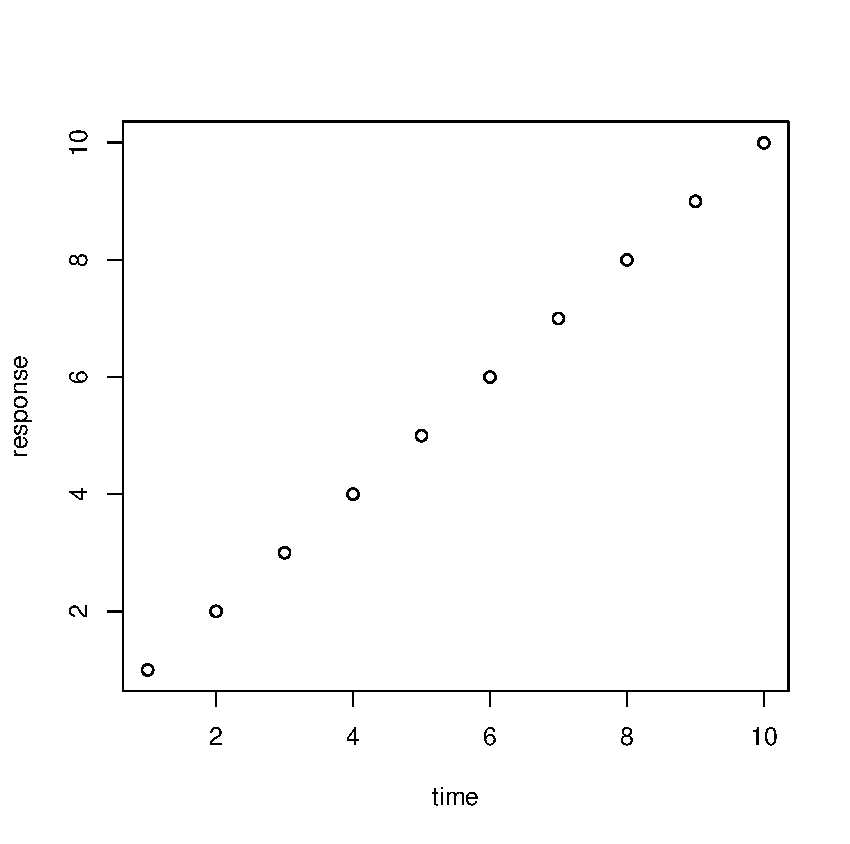
\includegraphics[width=3in]{fig1.pdf}
% \end{center}
% \caption{Consistency comparison in fitting surrogate model in the tidal
% power example. \label{fig:first}}
% \end{figure}

\section{Background and Related work}
\label{sec:meth}
Learning classifier System first used in \cite{10.1007/3-540-45712-7_54} but the basis of that experiment done with Wilson’s Zeroth level classifier system. In the following paper the author described the possibility of allowing suitable internal rule complexity to appear throughout learning and the structure reveals match set pattern as well as covering and its underlying features of the task, but in this paper  the application of self-adaptive mutation is inspired from the earlier work done by Bull \cite{111111111}. The paper from bull, tried to improve their act as devices for autonomous mobile robots using self-adaptive mutation. But with combining both self-adaptative and constructivist method a completely new work done in this following paper \cite{10.1145/1389095.1389364} and here it also used Zeroth-Level Classifier System (ZCS) as a base of their experiment used for real robot. Both paper (\cite{doi:10.1162/artl.2006.12.3.353},\cite{10.1007/3-540-45712-7_57}) came up with a common statement that in different situation or state it develops different solution for different kind of problem space. Another paper which is related to \cite{10.1145/1389095.1389364} uses a rule structure in which each is represented by an artificial neural network combining self-adaption \cite{111111111}, N-XCSF, Constructivism \cite{quartz_sejnowski_1997} (The complete overview is given in section 3.4) is applied to solve a complex environment. Although the author of this paper tried to focus on providing a generic solution in continuous environment, which is even more difficult than discrete environment space. The author also implemented connection selection that has been introduced earlier in \cite{10.1145/1388969.1389010} and that required another knowledge domain.

\section{Implementation}
\label{sec:1}



\subsection{Maze environment}
\label{sec:2}
\begin{figure}[!htbp]
\begin{center}
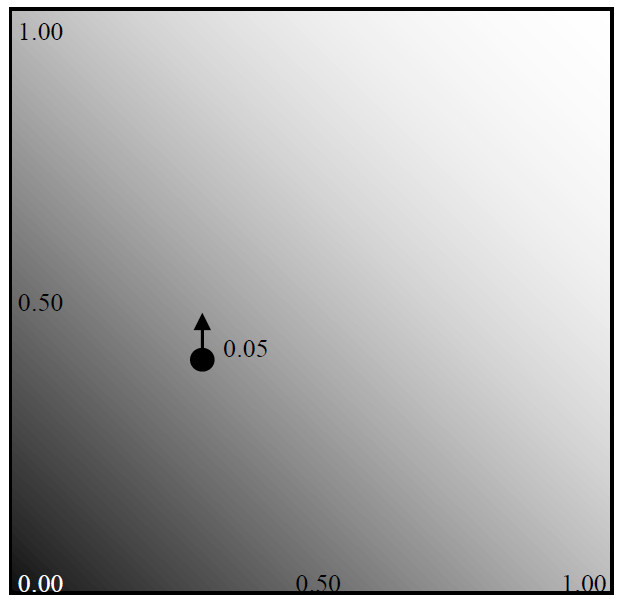
\includegraphics[width=3in]{fig_1.PNG}
\end{center}
\caption{The continuous 2D Grid environment, and a proposed agent movement (assuming discrete valued actions). \label{fig:first}}
\end{figure}
For the experimental space, the author chosen a complex test environment for the system. The 2-D continuous gridworld \cite{10.1007/978-3-540-30115-8_44} taking the state space into a 100 X 100 grid and the environment stretches from 0 to 1 in both directions as follows x and y and the agent initially starts at any random space with in this 100 X 100 grid except the goal state. The task of that agent is to get the goal state as less steps possible in the environment avoiding the obstacles. 
The agent uses a step size of 0.05 (Size of moving along to the goal state in action space) and the average size of reaching to the goal state is 21 as per the paper following\cite{111111111}. The agent obtains a reward of 1000 while hit the goal state and the discount rate $\gamma$ =0.95. Phototaxis is a commonly used task done by real robot to following the light gradient \cite{doi:10.1162/artl.2006.12.3.353}. The author of this paper proposed to use Phototaxis for a real robot to be following a light gradient to reach the goal state by fewest move possible. In \cite{doi:10.1162/artl.2006.12.3.353},\cite{10.1007/3-540-45712-7_57} more implementation and use of phototaxis is explained. As the author used MLP for this experiment but suggested to give a read to the single artificial neural network that evolution refer to this paper \cite{1554945} and the co-related work on NXCSF based on the 2-D Continuous gridworld problem can be found in this paper \cite{1554945}. 

\subsection{Neural XCSF (Discrete-valued actions)}
\label{sec:2}
Neural XCSF is a classifier system which introduced in the prediction estimation technique is used to learn an approximation of functions and finally the prediction is calculated. A remarkable generalization of classifier form is suggested in the following paper \cite{WilsonPrediction2001FunctionAW}.   
\begin{figure}[!htbp]
\begin{center}
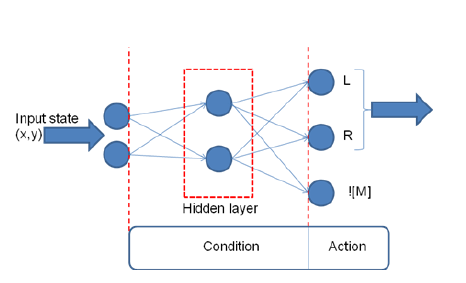
\includegraphics[width=6in]{fig_2.PNG}
\end{center}
\caption{Detailing the mapping between the condition of a traditional classifier and the MLP representation, and the computed action derived from the condition and the input state \label{fig:first}}
\end{figure}
The task of XCSF is to develop a population of classifiers which is denoted a [P] from the problem space. Every classifier of XCSF made of 2 components. Condition is one of them where most accurate conditions or rules are combined, and action is the response to that. In this paper a classifier is a Multi layered fully connected neural network that return calculated action and the condition as well. A match set [M] build in every iteration of XCSF from [P] which match the connection between [M] and [P] in every input state st which is basically the location of the agent in 2D Grid exact position value of x and y. But as compare to real world robot the position of x and y calculated +/- of (0 to 5) \% which is represented as noise in the real world compared to the grid position of the agent navigator. 


Initially a weight vector, $W_0$, which is initialized with 0 in every classifier and it compute the prediction. As this network has 2 input neuron it has 2 weight vector and additionally a $W_0$ which links to $X_0$ which is a constant parameter of XCSF function. When the match set [M] is evolved, a prediction which is a structure of Array is formed. The weight vector initialized previously with a 0 value and the output of XCSF is the input of environment respectively: 

% \lowercase{\mathcal{C} \mathcal{L\centerdot \mathcal{P} \left(\mathcal{S} \mathcal{T} \right) }
% $\Delta w_i = \eta / | X_(t - 1)|$
\begin{center} $cl.p(st) = cl.W_0*X_0 + \sum_{i>0} cl.w_i*st(i)$
\end{center}
The match set [M] does a cross check with correct set [C] for the given possible moves. The final action taken by the result of prediction array in regular XCSF to take the next step. In this whole process a newly formed delta rule has been introduced. In traditional XCSF the weight vector update with the classifier’s prediction value with this equation 1. But here with the use of delta rule the vector x is the state st and the parameter of XCSF function $X_0$ presents: 

\begin{center} $\Delta w_i = \eta / |X_{t - 1}|^2(r-cl.p(s_{t-1}))X_{t-1}$
\end{center}

\begin{center} $\varepsilon \leftarrow \varepsilon + \beta (| r-cl.p(S_{t-1}|-\varepsilon )$
\end{center}
If an action selected from the action set [A] and it reached to its goal state, the action gets a reward from the environment system. After getting the rewards it updates the parameter in action set[A]. In return the previous action[A-1] gets and discount if it really exists in action set. More about this updating parameter of XCSF described in \cite{WilsonPrediction2001FunctionAW}.
[P] $\rightarrow$ [M] $\rightarrow$ [A] is called trial.  The trial start with the randomly initialize the starting position in any action space. From that random position to reach in the goal state the trial takes ( [M]$\rightarrow$ [A] ) steps. It takes 2000 trial to complete the whole experiment by author.

\subsection{Self Adaptation }
\label{sec:2}
Among the various evolutionary computing technique self-adaptation is one of the well know technique. The author applied self-adaptation technique to maintain the amount of search to update the parameter in the environment.  GA trigger after a certain time in [A] to get the best outcome from the environment. A fully self-adaptive system presented, stepping ahead with that work author set $\mu$ value of every classifier randomly between 0 to 1 and the result also added in that range. The update version of the equation while mutation given below: 


\begin{center} $\mu \leftarrow \mu * e ^ {N(0,1)} $
\end{center}

\subsection{Neural constructivism }
\label{sec:2}
The term ‘Constructivism’ is a theory, that a learner learns anything based on their experience and the knowledge they had before about the learning topic. In neural network, same idea used for learning a model, the application of neural constructivism is a way of taking small sized network instead of taking a large sized network and work consistently with the small network. The small network gets updated for a long time updating/growing/pruning and again by deleting the extra features it gets better after a certain time and reached to an adequate level.
Constructivism has been introduced exactly the way (\cite{10.1007/3-540-45712-7_54},\cite{doi:10.1162/artl.2006.12.3.353}) got its way around and each rule consists of different number of hidden rules which is initially set to 1 and checked always the value should be greater than 0. After a successful GA cycle when the environment rules get updated constructivism applied there so that it can be normalize in a range. Apart from previous parameter two more parameter added $\psi$ (which shows the probability of completing constructivism) and another one is $\omega$ (Which denotes to the probability of adding a new neuron to the environment as well as the removal one in $\omega-1$). But both values initialize randomly between the range of 0 to 1. 
The author showed the result of the self-adaption in sections 3.3 and 3.4 that merge in two possible way (\cite{10.1007/3-540-45712-7_54},\cite{doi:10.1162/artl.2006.12.3.353}). 
\subsection{Connection selection }
\label{sec:2}
A neural network parameterizes with a lot of features which includes the most important one as well the least important one. Feature selection process is one kind of way to eliminate the least important of noisy feature of that network. Traditionally this can be done by any human being who has expert level of knowledge in this domain. But the problem with that it will take a long time, more effort and most important human can do several mistakes that can be run to the whole network into a less effective. For solving this problem, a method has been introduced earlier called ‘Wrapper’ method.  In wrapper method, GA cycle explore probabilistically rotate the connection to disable to enable or the other way around which is given to the learning and the learner gets only those useful features. In \cite{10.1145/1068009.1068210} the implementation of wrapper method done with a NEAT framework (FS-NEAT) with balancing 256 inputs.The author found this method less effective so another approach which is been implemented in \cite{10.1145/1388969.1389010} use in this paper called Boolean flag flipping. In GA cycle the classifier condition has a Boolean flag attached and based on self-adaptive parameter Tao the flag rotate from true to false or way around. For a new node the flag value always set to 0.5 and after changing the flag value being false to true results in randomly setting the value in range of 0 to 1. 


\section{Experimentation}
\label{sec:verify}
The author experimented each trial 20,000 times. The parameters were used are $\mathcal{N}$=16000, $\varTheta  _{DEL} $=50, $\beta$=0.2, $\varepsilon _{0}$=0.005, $\sigma $=0.1, $\mathcal{V}$=5, $\varTheta  _{GA} $=50 [31]. x0 [constant value] = 1, $\eta$[correction rate]  = 0.2, initial prediction error  = 0.01, and fitness to 10.0 for $X_0$. Every time a full one exploration cycle and one exploitation cycle occurs in the trial.Total 10 times the experiment checked, and the result were average. 
\section{Discrete-valued actions}
\label{sec:verify}
As in this section the NXCSF, is going through the process of discrete valued action the outputs of first two neuron which are real number and those values mapped with the real life discreate directions which are (East, West, North, South). As there are only two output possible the valued are discrete and range to 0.5 to 1 which means the value of x: 0.5$\leq$x$\leq$1(low) as well as for y: 0.5$\leq$y$\leq$1 (high). With the possibility of 2 output and 4 discrete direction the possible movement possible by the agent is (high, high) = North, (low, low) = West, (high, low) = East, (low, high) = south. In this paper, the author discussed about the existence of every action in [M] in the discrete action case. 

In figure 3a(left), It can be clearly shown while initially around 600 trial the value was far away from the optimal value but after nearly 650 it started finding the optimal solution but after around 7000 trial it gets its optimal value and later it kept going nearly with the same value.

In the following figure 3b(left),  it is shown that  the average number of hidden layer the author initialize with 1 as describe above but after around 7500 trial the average number of hidden layer increased to 1.8 or nearly 2 .Additionally from 6000 to final trial 20000 the value was quite stable and fluctuate around 1.5 to 2 but near the end of the trial around 16000 to 18000 there is a major fluctuation found in the  figure 3b. It clearly shows that the system solved the solution after 7500 trial but it still was searching for best possible solution so there was a major fluctuation happened near to the end.

In figure 3c(left), $\mu$, $\psi$, $\omega$ and $\tau$ value observed where self-adaptive $\mu$ reacts to this interruption as like 3b(left) and a huge change or fluctuation can be seen in around 18000 to 19500. With the help of connection selection this complex problem can be solve up to 20\% less connection needing compute per trial \cite{10.1145/1068009.1068210}. 

\begin{figure}
\begin{center}
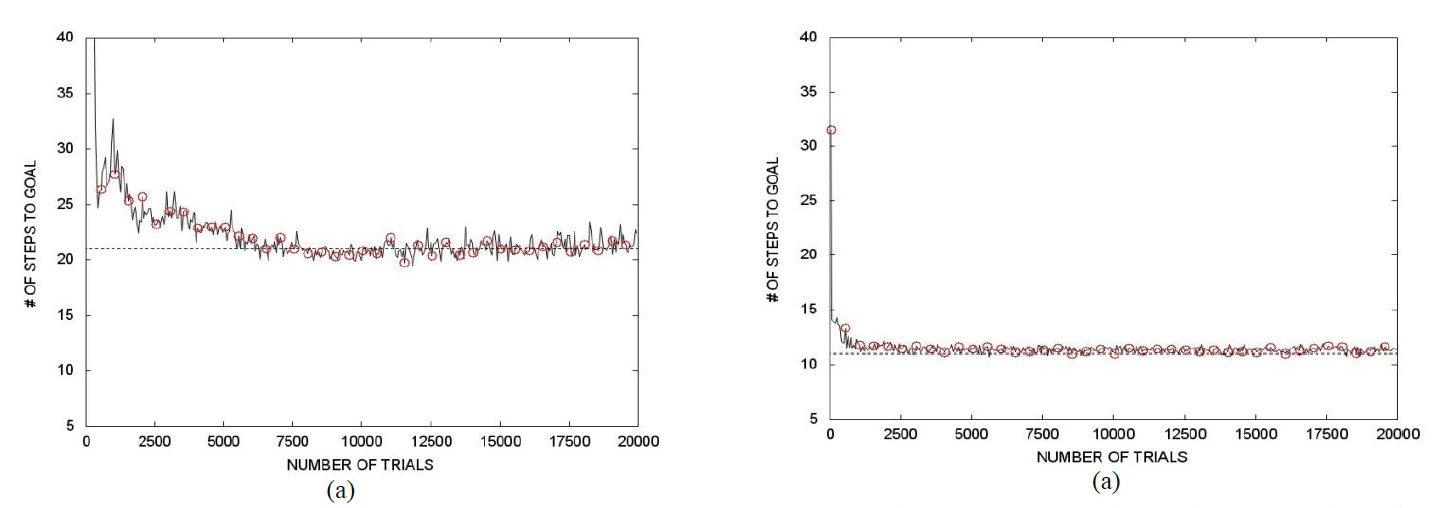
\includegraphics[width=6in]{3a.png}
\end{center}
\begin{center}
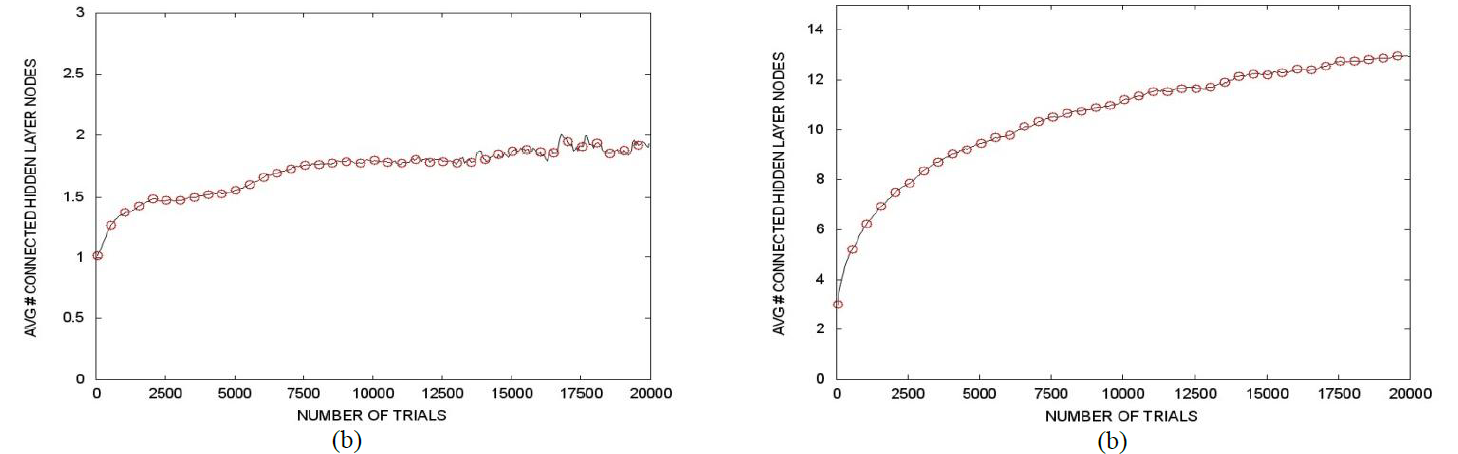
\includegraphics[width=6in]{3b.png}
\end{center}
\begin{center}
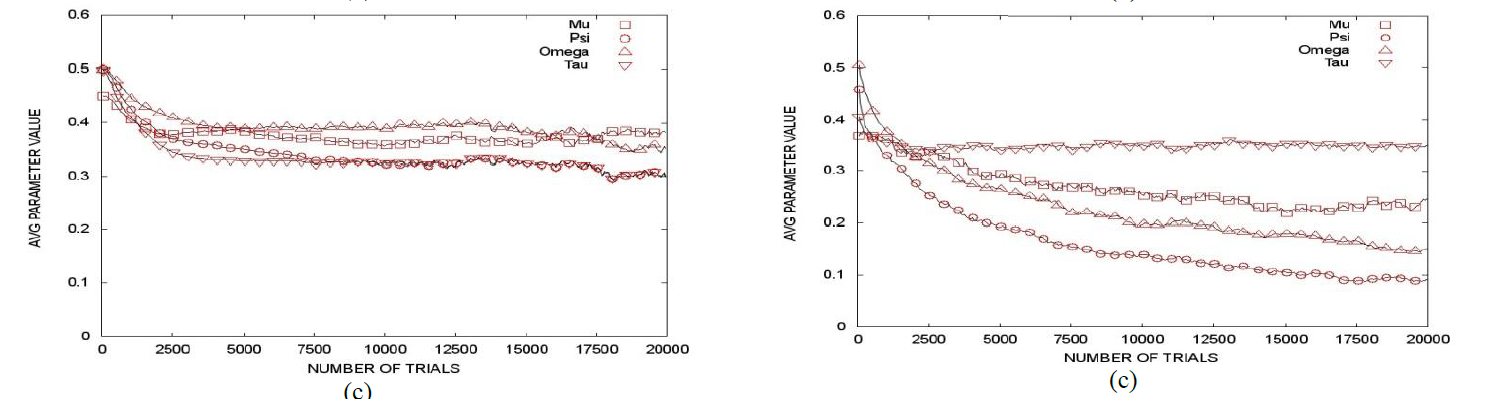
\includegraphics[width=6in]{3c.png}
\end{center}
\begin{center}
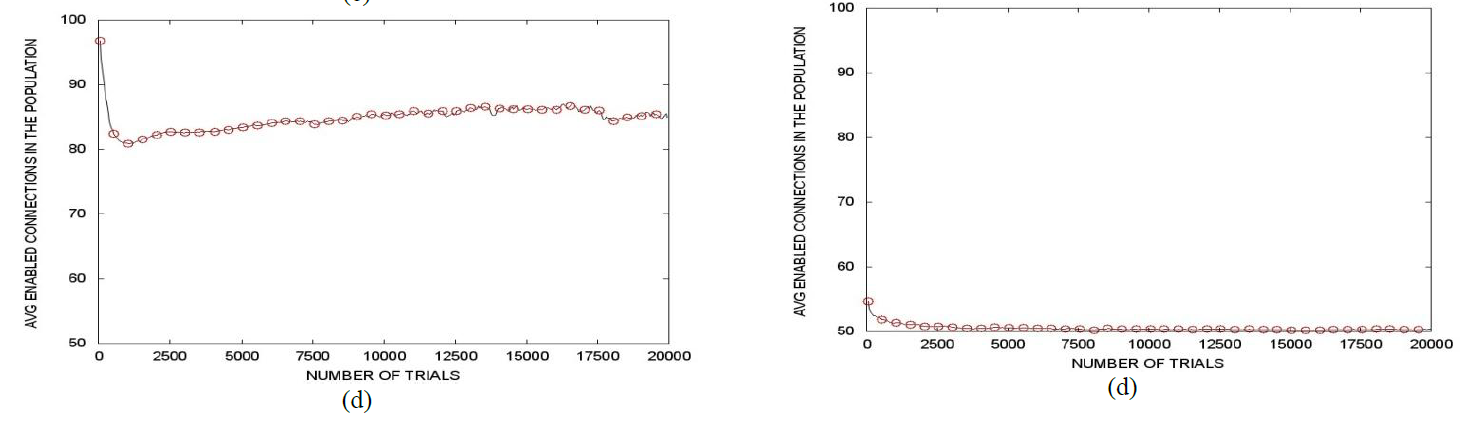
\includegraphics[width=6in]{3d.png}
\end{center}
\caption{Discrete-action N-XCSF (On Left) , Continuous-action N-XCSF (On Right) \label{fig:first}}
\end{figure}


\section{Continuous-valued actions}
\label{sec:verify}
Continuous valued action is the connection bridge between the real robot and an agent simulation. This paper has taken a drastic move after adding continuous-valued actions in the system. For discreate-valued action to the MLP the agent gets only 4 direction to move along. East, west, north, south is the four option but after applying continuous-valued action the agent gets a real number. As only four options in discrete-valued action leads to a limitation point for the system to reach the goal state with a optimal solution. Continuous-valued action gave the agent to move along any direction with almost highest of 6 dimension real numbered value to search for a optimal solution for the system. This kind of work with continuous-valued action previously done using XCSF but that originally applied \cite{WilsonPrediction2001FunctionAW} the starting version of NXCS. Vague logic used for the first time \cite{10.11415/1276958.1277327} after that in \cite{10.1007/3-540-45027-0_5} and lastly in XCS \cite{4286961}. To control a robot arm very recently \cite{10.1145/1389095.1389360} XCSF used. Current arm posture for a robot to move have been done by this. The input section determines the arm angle for the rotation in degree and the prediction encodes changes the hand location in left or right direction \cite{349978}. 

With the idea of those previous paper the author changed a bit in this paper. The implementation of this method is done by taking the output of each MLP node and setting the real value to be normalize between [-0.05 , 0.05]. As the Output has three value those refer to movement in X direction movement in Y direction and lastly the match set. First 2 nodes combine the value from -0.05 to 0.05 and combining them the agent get a direction to move. [M] formation created and a single classifier picked from [A]. Initially the covering mechanism set to a 0 vector and by time it sets its prediction rules. All the agent’s located in a ra random value between 0 to 1 and now assumed the steps-to-goal for this environment reduced to 11 from 21.

Figure 3a(right) shows that initially it started around 32 steps-to-goal but after almost 800 trials the value got down to 12-14. Within 1500 trial the value was in 11 of nearly 12 and it kept the same in the whole 20000 trial. If we compare with the discreate-value in 3a(left) we can clearly see the difference between 21 and 11 step-to-goal value and here thanks to the neural XCSF linear prediction.

The comparison between 3b(right) and 3b(left) shows the change of hidden layer nodes in different trial.  In continuous-valued action 3b(right) shows the average number of hidden layer increase gradually from 2.5 to nearly 13 with in around 600 trials. On the other hand in discrete-valued section fig 3b(left) after almost 25000 trials the average hidden layer gone up to 2. The increment of hidden layer is arise the problem complexity of the system. 

The changes in the final $\mu$ value seen in fig 3c(right) and 3c(left) showed slide different result in the same environment. This is a sign that self-adaptation method can vary from time to time and change in different environment with different valued which is depend on the position of the agent in the environment. Finally, the result shows that after almost 500 trial the number of enable connection is the population get to around 55 and later is constantly gave the same value around 50. In real life as well as this paper is shows that one network generally controls all the actions for the environment to move along with.


\section{Continuous-Duration actions}
\label{sec:verify}
\begin{figure}[!htbp]
\begin{center}
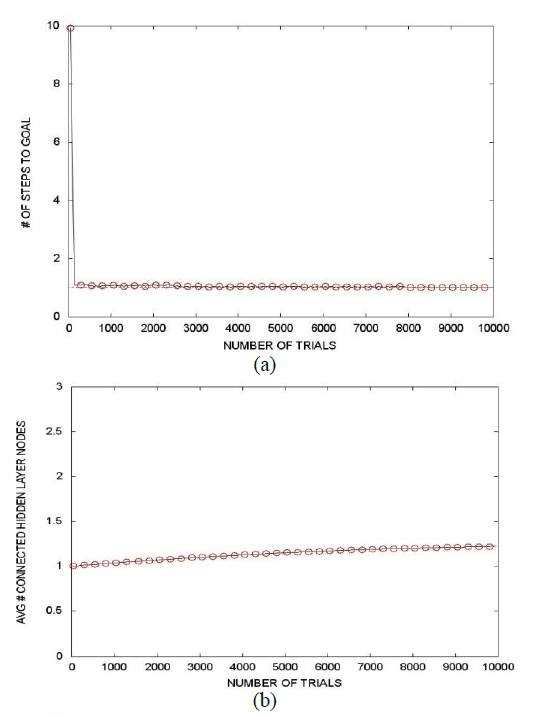
\includegraphics[width=3in]{5a.png}
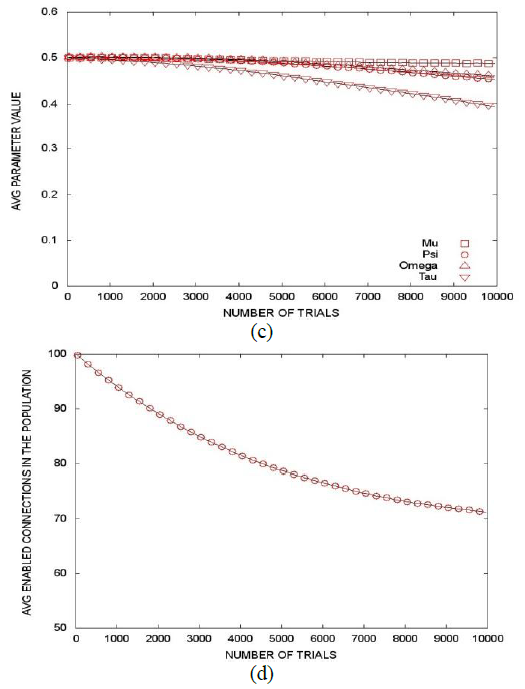
\includegraphics[width=3in]{5b.png}
\end{center}
\caption{Continuous-duration action N-XCSF (a) steps to goal (b) average connected hidden layer nodes in [P] (c) self-adaptive parameter values (d) average enabled connections in the population \label{fig:first}}
\end{figure}
Continuous-duration actions is another step as before explained continuous-valued action, is also the connecting bridge of real robot and simulation. The logic of using this is not to limit the agent in single steps, despite updating the parameter and set the action set [A] in the environment for continuous time. Previously several works done regarding this and the author suggested to read \cite{349978} to the readers. The system in this paper laid on ‘temporal’ LCS which has been used in several places. The concept is same as before [M] is the matching set and [A] is the action set. But the process is bit different from the original LCS. In TCS the [A] is formed by the state of the agent but while roaming to the environment the agent does not inform [M] to mutate the matching set. Matching all classifier in [A] results in taking next move in to count. In the opposite situation the action is dropped from the environment and a newly match set [M] formed. But matching some classifier splits the [A] in to two more set [C] and [D]. If it is [C](continue) then it removes [D] classifiers from [A] on the other hand if it is [D](drop current), [A] results in removing [C] classifiers from [A] and new [M] formed. 

\begin{center} $ P  = r  + \gamma * maxP$
\end{center}
\begin{center} $ P  = (e ^ {-\varphi t^t})r  + (e ^ {- pt^i})r * maxP$
\end{center}
In the formula r, $\gamma$, maxP stand for reward, discount factor and maximum prediction array respectively. Slightly breaking the equation new term introduced in the paper $e ^ {-\varphi t^t}$ and $e ^ {- pt^i}$ as a first and second reward factor and implementing it the author described the classier [A] is always the same.For this reason, the concept of splitting [A] in to more 2 [C] and [D] was not needed here. As describe above the system implemented by author does not reform [M] match set after each cycle it can reach to its goal state without doing that. Temporal Learning System used here with all the value keeping same as before just changing the trial amount 20000 to 10000.From the fig 4 the optimality for this environment got very rapidly.
\section{Conclusion}
\label{sec:conc}
In conclusion of this paper, it is shown that adding continuous-valued and continuous-duration to the environment it reflects the same outcome as real robot shows as well as the simulation and this concept can be implemented successfully. Continuous-duration can be used for improving the performance of any LCS environment. Also, a self-adaptive neural network with constructivism in it efficient enough to solve a complex 2D grid environmental problem with an optimal number of moves.

The author suggested(extension), of this work can be done by adding more complex obstacle in the environment for the agent to reach the goal state so that the agent can get more complex grid environment such as Puddles environment \cite{1554945} to work on and get the optimal solution.

Finally, By the time of publishing the paper(This paper published in 2009), according to the author this is the first modern concept they have implemented the reinforcement learning within an LCS environment and the process consists of continuous-valued action in reaction of continuous-valued input.

% \medskip
% %Bibliographic references
% \begin{thebibliography}{9}
% \bibitem{inproceedings} 
% \end{thebibliography}

\bibliographystyle{unsrt}

\bibliography{Bibliography-MM-MC}



\end{document}

